\section{Appendix}

\begin{frame}{Notation}
\begin{itemize}
\item $X,Y,Z$: (subsets of) random variables.
\item $\mathcal{X} = (X_1,\ldots,X_n)$: all random variables of a PGM.
\item $G = (\mathcal{X},A)$: Bayesian network.
\item $H = (\mathcal{X},E)$: Markov network.
\item $Z$: Partition function of Gibbs distribution.
\item $\Phi,\phi$: All factors/factor of a Gibbs distribution.
\item $\Pb_{\Phi}, \tilde{\Pb}_{\Phi}$: normalized/unnormalized Gibbs distribution over factors $\Phi$.
\item $\epsilon$: energy function (logarithm of factor) of a Gibbs distribution.
\item $\mathcal{I}(\Pb)$: All conditional independencies holding for prob.\ distr.\ $\Pb$.
\item $\mathcal{I}_l(G)$: Local conditional independencies of Bayesian network $G$.
\item $\mathcal{I}(G)$: Global (d-separation) conditional independencies of Bayesian network $G$.
\item $\mathcal{I}_h(H)$: Pairwise conditional independencies of Markov network $H$.
\item $\mathcal{I}_l(H)$: Local conditional independencies of Markov network $H$.
\item $\mathcal{I}(H)$: Global (separation) conditional independencies of Markov network $H$.
\item $\mathcal{I}_{\Phi,\prec}$: Induced graph of a factorization $\Phi$ and elimination ordering $\prec$.
\end{itemize}
\end{frame}

\begin{frame}{Graphs}
\begin{definition}[Parents]
$A$ is a parent to $B$ in a directed graph $\mathcal{G}=(\mathcal{V},\mathcal{A})$ if $A \rightarrow B \in \mathcal{A}$.
We call $\Pa{\mathcal{G}}{B}$ the set of parents of $B$.
\end{definition}
%
\begin{definition}[Ancestors, Descendants]
$A$ is an ancestor of $B$ (resp.\ $B$ is a descendent of $A$) in a directed graph $\mathcal{G}=(\mathcal{V}, \mathcal{A})$ if there exists a directed path $A = X_1 \rightarrow X_2 \rightarrow \ldots \rightarrow X_k = B$, $X_i \rightarrow X_{i+1} \in \mathcal{A}$ $\forall i \in [k-1]$.

We call $\Anc[A]$ the set of ancestors of $A$
and $\Desc{A}$ the set of descendants of $A$.
\end{definition}
%
\begin{definition}[Non-Descendants]
$A$ is a non-descendant of $B$ in a directed graph $\mathcal{G}=(\mathcal{V}, \mathcal{A})$ if $A \in \mathcal{V} \backslash \Desc{B}$. 
We call $\ND{\mathcal{G}}{B}$ the set of non-descendants of $B$.
\end{definition}
%
\begin{definition}[Neighbors]
    The set of neighbors of a node $A$ is $\Nb(A) = \{B : \text{there exists an edge } A-B\}$.
\end{definition}
\begin{definition}[Topological Ordering]
$X_1,\ldots,X_n$ is a topological ordering of a directed graph $\mathcal{G}=(\mathcal{V},\mathcal{A})$ if $\mathcal{V} = \{X_1,\ldots,X_n\}$ and $X_i \rightarrow X_j \in \mathcal{A} \Rightarrow i < j$.
\end{definition}
\end{frame}

\begin{frame}{Probabilistic Concepts}
\begin{description}
    \item[Conditional Probability:]
    \begin{equation}
        \Pb[X|Y] = \frac{\Pb[X,Y]}{\Pb[Y]}
    \end{equation}
    \item[Chain Rule:]
    \begin{equation}
        \Pb[X_1,X_2,\ldots,X_k] = \Pb[X_1] \Pb[X_2 | X_1] \cdots \Pb[X_k | X_1,\ldots,X_{k-1}]
    \end{equation}
    \item[Bayes Rule:]
\begin{equation}
    \Pb[X|Y] = \frac{\Pb[Y|X]\Pb[X]}{\Pb[Y]}
\end{equation}
\item[Independence] of two random variables $X$ and $Y$ is given by
\begin{equation}
    X \indep Y \Leftrightarrow \Pb[X,Y] = \Pb[X] \Pb[Y]
\end{equation}
\item[Conditional Independence] of two random variables $X,Y$ conditioned on $Z$ is given by
\begin{equation}
    X \indep Y | Z \Leftrightarrow \Pb[X,Y|Z] = \Pb[X|Z] \Pb[Y|Z]
\end{equation}
\item[Kullback-Leibler Divergence]
\begin{equation}
KL(P,Q) = \int_{x \in \mathcal{X}} P(x) \log\left(\frac{P(x)}{Q(x)}\right) dx
\end{equation}
\item[Mutual Information]
\begin{equation}
I(P,Q) = KL(\mathbb{P}_{XY}, \mathbb{P}_X \cdot \mathbb{P}_Y)
\end{equation}
\item[Mutual Information $\leftrightarrow$ Independence] $I(X,Y) = 0$ if and only if $X \indep Y$.
\end{description}
\end{frame}

\begin{frame}{Independence, Correlation}
    \label{appendix:correlation-independence}
    \begin{columns}[t]
        \column{0.5\textwidth}
        \textbf{Pearson's Correlation}
\begin{itemize}
    \item Normalized Covariance:
\begin{equation}
    \rho(X,Y) = \frac{\Cov{X,Y}}{\sqrt{\Var{X}} \sqrt{\Var{X}}}
\end{equation}
\item Captures linear dependency

\end{itemize}
    \hfill\vrule\hfill
\column{0.5\textwidth}
\textbf{Independence}
\begin{itemize}
    \item Joint distribution factorizes:
     \begin{equation}
        X \indep Y \Leftrightarrow \Pb[X,Y] = \Pb[X] \Pb[Y]
     \end{equation}
\end{itemize}
\end{columns}

\hrule
\begin{center}
\textbf{Properties:}
\begin{itemize}
    \item $X \indep Y$ implies $\rho(X,Y) = 0$.
    \item $\rho(X,Y) = 0$ does not imply X $\indep Y$ (except for Gaussians). 
\end{itemize}
\end{center}

\hrule
\begin{columns}
\column{0.5\textwidth}
%\textbf{Partial Correlation (for Gaussians)}
%\begin{itemize}
%    \item Correlation measured after eliminating linear effect of conditional variable 
%    \begin{equation}
%        \rho(X,Y | Z) = 
%    \end{equation}
%\end{itemize}
%\column{0.5\textwidth}
\textbf{Conditional Independence}
\begin{itemize}
    \item Joint conditional distribution factorizes:
    \begin{equation}
       X \indep Y | Z \Leftrightarrow \Pb[X,Y|Z] = \Pb[X|Z] \Pb[Y|Z]
    \end{equation}
\end{itemize}
%\end{columns}
\hfill\vrule\hfill
\column{0.5\textwidth}
%\hrule
\begin{center}
\textbf{Properties:}
\begin{itemize}
    \item $X \indep Y | Z$ implies $\rho(X,Y|Z) = 0$.
    \item $\rho(X,Y|Z) = 0$ does not imply X $\indep Y|Z$ (except for Gaussians). 
\end{itemize}
\end{center}
\end{columns}
\end{frame}

\begin{frame}{Conditional Independence Properties}
    \label{appendix:conditional-independence-properties}
\begin{description}
    \item[Symmetry] 
    \begin{equation}
        (X \indep Y | Z) \Leftrightarrow (Y \indep X | Z)
    \end{equation}
    \item[Decomposition] 
    \begin{equation}
        \label{eq:decomposition-property}
        (X \indep Y,W | Z) \Rightarrow (X \indep Y | Z)
    \end{equation}
    \item[Weak Union]
    \begin{equation}
        (X \indep Y,W | Z) \Rightarrow (X \indep Y | W, Z)
    \end{equation}
    \item[Contraction]
    \begin{equation}
        (X \indep W | Y, Z) \text{ and } (X \indep Y | Z)  \Rightarrow (X \indep Y, W | Z)
    \end{equation}
\end{description}
\begin{definition}[Positive Random Variable]
    A random variable if called positive, if 
    \begin{equation}
        \Pb[X = x] > 0 \quad \forall x 
    \end{equation}
\end{definition}
\begin{description}
    \item[Intersection] Let $X,Y,Z,W$ be jointly positive random variables. Then
    \begin{equation}
        \label{eq:intersection-property}
       (X \indep Y | W,Z) \text{ and } (X \indep W | Y,Z) \Rightarrow (X \indep Y,W | Z) 
    \end{equation}
\end{description}
\end{frame}

\begin{frame}{Laws of Large Numbers}
\begin{theorem}[Strong Law of Large Numbers]
Let $X^i \sim \Pb[X]$, $i \in \N$ be iid real-valued random variables such that $E_{\Pb}[X]$ exists.
Then
\begin{equation}
    \lim_{n \rightarrow \infty} \frac{1}{n} \sum_{i=1}^n X^i = \E_{\Pb}[X] \quad \text{almost surely}
\end{equation}
\end{theorem}
\begin{theorem}[Central Limit Theorem]
Let $X^i \sim \Pb[X]$, $i \in \N$ be iid real-valued random variables such that $\E_{\Phi}[X^i] = \mu$ and $\Var{X^i} = \sigma^2$. 
Then
\begin{equation}
    \lim_{n \rightarrow \infty} \Pb[\frac{\sum_{i=1}^n X^i - \mu}{\sqrt{M} \cdot \sigma} < r] = \Phi(r) \,,
\end{equation}
where $\Phi(r) = \Pb[Z < r]$ and $Z \sim \mathcal{N}(0,)$ is a random Gaussian variable.
\end{theorem}
\end{frame}


\begin{frame}{Probabilistic Language}
\begin{description}
    \item[Inference, Probability Queries:] Answer queries using the distribution as model.
    \begin{description}
    \item[Evidence, Observation:] Typically denoted by random variable $E$ or $O$, values that are observed.
    \item[Query Variables:] Typically denoted by random variable $X$, probable states that we want to infer.
    \item[Marginal MAP, Posterior Distribution:]
    \begin{equation}
        \Pb[X|E] = \frac{\Pb[X,E]}{\sum_{X}\Pb[X,E]}
    \end{equation}
    \item[MAP, Maximum-A-Posteriori:] 
    \begin{equation}
    \max_{X} \Pb[X | E]
    \end{equation}
    \end{description}
\end{description}
\end{frame}

\begin{frame}{Constrained Optimization, Lagrangian}
\begin{minipage}{0.49\textwidth}
\textbf{Unconstrained Optimization}
\begin{itemize}
    \item \underline{Stationary Points:} Compute $\min_{x} f(x)$ by searching points with $\nabla f(x) = 0$.
\end{itemize}
\end{minipage}
\begin{minipage}{0.49\textwidth}
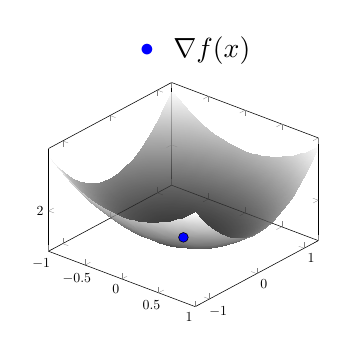
\begin{tikzpicture}[scale=0.5]
\begin{axis}[view={40}{40}]
%\addplot3[fill=magenta, opacity=0.5] coordinates{ (-1,-1,1) (-1,1,1) (1,1,1) (1,-1,1) };
\addplot3[ surf, colormap/blackwhite, opacity=0.8, shader=interp, domain=-1:1, domain y=-1.3:1.3, ] {+x^2+y^2+1};
%\addplot3[->, blue, very thick] coordinates {(0,0,1) (0,0,1.01)};
\addplot3[only marks, mark=*, mark size=3.5, mark options={fill=blue}] coordinates {(0,0,1)};
\end{axis}
% legend
\node at (2.5,6.5) [label=right: $\nabla f(x)$] {\textcolor{blue}{$\bullet$}};
\end{tikzpicture}
\end{minipage}
\hrule
\begin{minipage}{0.49\textwidth}
\textbf{Constrained Optimization}
\begin{itemize}
    \item \underline{Stationary Points:} Compute $\min\limits_{x : g(x) = 0} f(x)$ by searching points with $\nabla f(x) + \lambda \nabla g(x) = 0$.
    \item \underline{Intuition:} The gradient $\nabla f(x)$ must be orthogonal to the subspace $\{x : g(x) = 0\}$.
\end{itemize}
\end{minipage}
\begin{minipage}{0.49\textwidth}
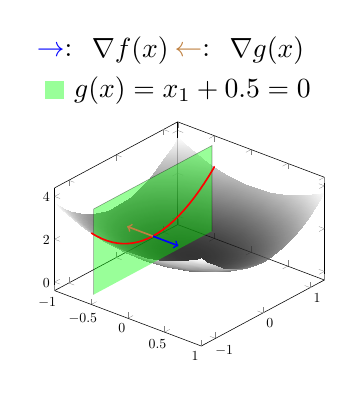
\begin{tikzpicture}[scale=0.5]
\begin{axis}[view={40}{40}]
\addplot3[ surf, colormap/blackwhite, opacity=0.8, shader=interp, domain=-1:1, domain y=-1.3:1.3, ] {+x^2+y^2+1};
\addplot3[fill=green, opacity=0.4] coordinates{ (-0.5,-1.25,0) (-0.5,-1.25,4) (-0.5,1.25,4) (-0.5,1.25,0) };
\addplot3[red, very thick, domain=-0.5001:-0.4999, domain y=-1.3:1.3, ] {+x^2+y^2+1};
\addplot3[->, blue, very thick] coordinates {(-0.5,0,0.25+1) (-0.15,0.0,0.25+1)};
\addplot3[->, brown, very thick] coordinates {(-0.5,0,0.25+1) (-0.85,0.0,0.25+1)};
\end{axis}
% legend
\node at (0,7.5) [label=right: $\nabla f(x)$] {\textcolor{blue}{$\rightarrow$}:};
\node at (3.5,7.5) [label=right: $\nabla g(x)$] {\textcolor{brown}{$\leftarrow$}:};
\node at (0,6.5) [fill=green, opacity=0.4, label=right:{$g(x) = x_1 + 0.5 = 0$}] {};
\end{tikzpicture}
\end{minipage}
\end{frame}

\begin{frame}{Fixed Point Theorem}
\begin{theorem}[Banach's Fixed Point Theorem]
Let $C$ be a compact space and $d$ a metric on $C$. Let $F$ be a strict contraction, i.e.\ there exists $\alpha \in [0,1)$ such that
\begin{equation}
   d(F(x), F(y)) \leq \alpha d(x,y) \quad \forall x,y \in C\,.
\end{equation}
Then $F$ has a unique fixed point $z \in C$ (meaning $F(z) = z$) and
\begin{equation}
    \lim_{n \rightarrow \infty} F^n(x) = z \quad \forall x \in C\,.
\end{equation}
\end{theorem}
\end{frame}